% ================================================================ 3.7
% RLAIF / Constitutional AI (de-duplicated to ONE diagram with overlays)
\begin{frame}{Scaling Oversight: RL from AI Feedback (RLAIF)}
\begin{itemize}\itemsep0.3em
    \item \textbf{Motivation:} as models approach or exceed human performance, it
          gets harder for humans to label every output. \emph{Move the labeller
          from human to AI; the only human input is the constitution}, a short
          list of written principles the model uses to critique and revise its own
          answers.
    \item \textbf{Constitutional AI} has two phases:
    \begin{itemize}\footnotesize
        \item \textbf{Supervised:} sample $\to$ self-critique $\to$ revise $\to$
              fine-tune on revisions.
        \item \textbf{RL:} AI labels which response is better $\to$ train a
              reward model (RM) $\to$ RL-finetune with it (just like RLHF).
    \end{itemize}
\end{itemize}
\vfill
\begin{center}
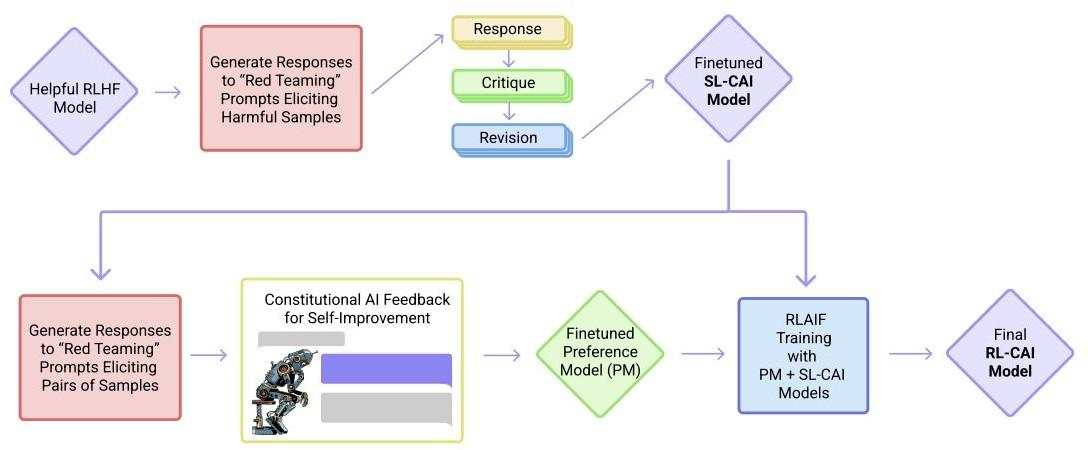
\includegraphics[width=0.78\linewidth, height=0.32\textheight, keepaspectratio]{images/rl-real-world/figures/cai-pipeline.jpg}
\end{center}
\srcnote{\scriptsize Bai et al. \href{https://arxiv.org/abs/2212.08073}{Constitutional AI: Harmlessness from AI Feedback}, 2022. In production, not a toy.}
\end{frame}

\begin{frame}{RLAIF: Takeaway}
\begin{itemize}
    \item Fine-tuning with \textbf{AI-generated feedback} can match or exceed
          models fine-tuned with human feedback, on \emph{both} helpfulness and
          harmlessness.
    \item \footnotesize The plot rates models by \textbf{Elo}, a head-to-head
          win-rate score borrowed from chess (higher = preferred more often in
          pairwise comparisons).
\end{itemize}
\vfill
\begin{center}
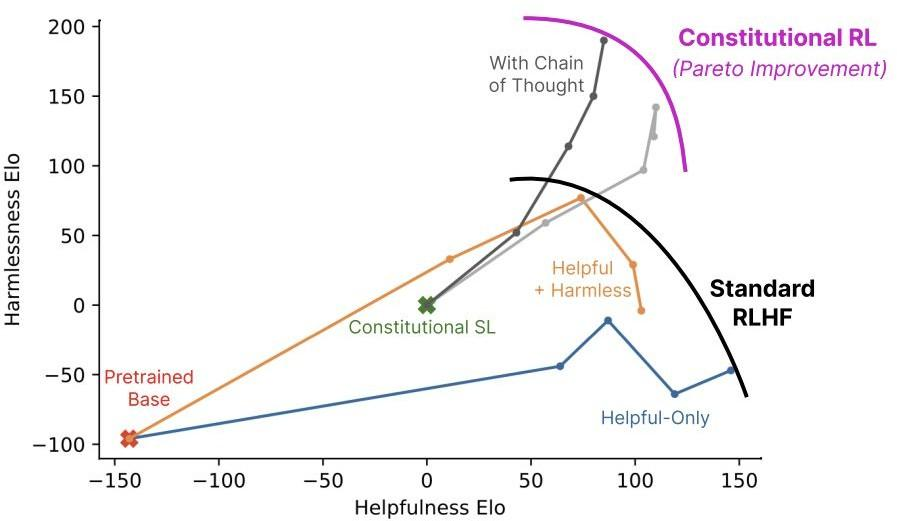
\includegraphics[width=0.55\linewidth, height=0.55\textheight, keepaspectratio]{images/rl-real-world/figures/rlhf-elo.jpg}
\end{center}
\end{frame}

% ================================================================ 3.8
% RLVR / RL for reasoning (NEW - the lecture's climax) - TikZ spectrum
\begin{frame}{The Climax: RL with Verifiable Rewards (RLVR)}
\begin{itemize}\itemsep0.3em\small
    \item When the answer is \textbf{checkable} (math is right/wrong, code
          passes tests), the reward needs \emph{no learned model} and
          \textbf{can't be hacked} the way an RM can.
    \item This is how modern \textbf{reasoning models} are trained: long
          \textbf{chain-of-thought} (the model writes out its reasoning steps before
          answering), optimized with \textbf{GRPO} against a programmatic check.
\end{itemize}
\vfill
\centering
\resizebox{0.98\linewidth}{!}{%
\begin{tikzpicture}[font=\footnotesize,
    stop/.style={draw, rounded corners, minimum width=3.0cm, minimum height=1.0cm, align=center},
    ar/.style={-{Stealth[length=2.4mm]}, very thick}]
  \node[stop, fill=boxtan]   (rlhf) at (0, 0)  {\textbf{RLHF}\\\scriptsize human prefs};
  \node[stop, fill=boxblue]  (rlaif)at (4.5, 0){\textbf{RLAIF}\\\scriptsize AI prefs};
  \node[stop, fill=mlgreen]  (rlvr) at (9, 0)  {\textbf{RLVR}\\\scriptsize verifiable};
  \draw[ar] (rlhf) -- (rlaif);
  \draw[ar] (rlaif) -- (rlvr);
  % reward source under each
  \node[font=\scriptsize, align=center, below=0.3cm of rlhf]  {learned RM\\(Bradley--Terry)};
  \node[font=\scriptsize, align=center, below=0.3cm of rlaif] {AI judge\\+ constitution};
  \node[font=\scriptsize, align=center, below=0.3cm of rlvr]  {programmatic check\\(answer / unit tests)};
  % annotation arrows
  \draw[-{Stealth[length=2mm]}, gray] (0, 1.4) -- node[above, font=\scriptsize]{scales better $\rightarrow$} (9, 1.4);
  \draw[-{Stealth[length=2mm]}, gray] (0, 0.9) -- node[above, font=\scriptsize]{harder to hack $\rightarrow$} (9, 0.9);
\end{tikzpicture}%
}
\srcnote{\scriptsize DeepSeek-AI, \href{https://arxiv.org/abs/2501.12948}{DeepSeek-R1}, 2025; Lambert et al., \href{https://arxiv.org/abs/2411.15124}{T\"ulu 3}, 2024 (RL with verifiable rewards).}
\end{frame}

% ---------------------------------------------------------------- 3.8b RLVR in action: R1-Zero
\begin{frame}{RLVR in Action: DeepSeek-R1-Zero}
\textbf{One RLVR step} (no reward model anywhere):
\begin{enumerate}\itemsep0.1em\small
    \item the policy samples several answers to a \emph{checkable} question;
    \item a \emph{rule} grades each (right answer? right format?), giving reward
          $1$ or $0$;
    \item GRPO uses those rewards to update the policy. \empr{Nothing to hack: the
          checker is exact.}
\end{enumerate}
\vspace{0.3em}
\textbf{DeepSeek-R1-Zero} ran exactly this on a \emph{base} model, \textbf{no SFT
at all}, with reward = ``answer correct'' $+$ ``reasoning in \texttt{<think>}
tags'':
\begin{itemize}\itemsep0.1em\small
    \item \empr{Reasoning emerged on its own}: longer chains of thought,
          self-checking, backtracking, even an ``\emph{aha moment}'' where it stops
          and corrects itself. Nobody taught it to.
    \item AIME 2024 math: \textbf{15.6\% $\to$ 71.0\%} (86.7\% with majority vote), matching OpenAI o1.
    \item Catch: raw R1-Zero was hard to read (language-mixing), so the full
          \textbf{R1} adds a small SFT ``cold start.'' But R1-Zero proved the point:
          \empr{reasoning can be grown by pure RL from verifiable rewards.}
\end{itemize}
\srcnote{\scriptsize DeepSeek-AI, \href{https://arxiv.org/abs/2501.12948}{DeepSeek-R1: Incentivizing Reasoning Capability in LLMs via Reinforcement Learning}, 2025.}
\end{frame}
